\documentclass[conference]{IEEEtran}

\usepackage{cite}
\usepackage{amsmath,amssymb,amsfonts}
\usepackage{algorithmic}
\usepackage{graphicx}
\usepackage{textcomp}
\usepackage{xcolor}
\usepackage{booktabs}
\usepackage{multirow}
\usepackage{url}
\usepackage{hyperref}
\usepackage{tikz}
\usepackage{pgfplots}
\pgfplotsset{compat=1.18}
\usetikzlibrary{arrows.meta, positioning, calc}

\setlength{\textfloatsep}{6pt plus 2pt minus 2pt}
\setlength{\intextsep}{6pt plus 2pt minus 2pt}
\setlength{\abovecaptionskip}{3pt}
\setlength{\belowcaptionskip}{0pt}

\begin{document}

\title{AgentModernize: Preserving Business Logic in Legacy Modernization with Multi-Agent LLMs and Behavioral Specification Graphs}

\author{\IEEEauthorblockN{Anonymous Author(s)}
\IEEEauthorblockA{Anonymous Institution\\Anonymous City, Country}}

\maketitle

\begin{abstract}
Legacy modernization routinely breaks business logic. Most tools and LLM-based approaches treat modernization as syntax translation: convert COBOL to Java, swap PL/SQL for Python, ship it. Implicit rules, edge-case handling, and cross-module constraints that keep production systems running are lost, and nobody notices until something fails in production.

We present \textit{AgentModernize}, a multi-agent framework that treats modernization as a behavioral preservation problem. Four agents handle extraction, specification, code generation, and validation. The key intermediate artifact, a \textit{Behavioral Specification Graph (BSG)}, forces extracted business logic to be explicit and inspectable before any code is generated.

We evaluated on LegacyModernize-8, eight synthetic COBOL scenarios, under a fair protocol where each method's tests are generated from its own API surface (3 trials, GPT-4o-mini). After an independent regeneration failed to reproduce our initial run, we report the new run as primary: a no-BSG feedback baseline scored the highest mean BER (12.4\%), ahead of the full pipeline (10.2\%), single-prompt (9.7\%), chain-of-thought (6.5\%), no-feedback (3.9\%), and a regression-aware variant (3.3\%). Feedback helped selectively (+22.2, +36.7 points on two scenarios), while Validator-generated tests proved a weak iteration-selection signal. The BSG captured 94.4\% of gold-standard rules at 93.0\% precision against $\leq$13\% end-to-end BER for every method: extraction works, generation is the bottleneck. We conclude the BSG's value is as an inspectable, compilable specification artifact---required for enterprise estates too large for any prompt---not as a BER multiplier, and that single-generation-draw results in this domain are unreliable.
\end{abstract}

\begin{IEEEkeywords}
legacy modernization, multi-agent systems, large language models, business logic preservation, behavioral equivalence, software engineering
\end{IEEEkeywords}

%% ============================================================
\section{Introduction}

Telecommunications carriers, financial institutions, and healthcare providers run their core operations on systems built twenty or thirty years ago. COBOL batch jobs process billing. PL/SQL procedures enforce contract logic. Shell scripts orchestrate provisioning workflows. These systems work, and the business rules encoded in them have been refined through years of production experience, bug fixes, and regulatory adaptation~\cite{comella2000survey}. They are also expensive to maintain, difficult to integrate with modern platforms, and increasingly fragile as the engineers who wrote them retire~\cite{breivold2012systematic}.

Modernization is the standard response, but most modernization efforts destroy the thing they should preserve: behavioral semantics. Business rules in legacy systems are rarely documented; they live in control flow patterns, conditional branches, exception handlers, and configuration files~\cite{kazman1998requirements}. A line-by-line COBOL-to-Java translation can compile and run yet silently break edge-case handling, alter validation logic, or drop constraints that were never written down~\cite{rugaber2004model}. We saw this firsthand in a telecom provisioning workflow where a syntactically correct translation passed compilation but silently dropped a suspended-account exemption that had been in production for fifteen years. The system looked modern and behaved differently.

Large Language Models can parse legacy code, reason about intent, and generate modern equivalents~\cite{chen2021evaluating}, but prompting one to ``convert this legacy code to a modern API'' is brittle. Context windows cannot hold an entire legacy codebase; a single generation pass provides no way to verify behavior was preserved; and a monolithic prompt conflates understanding, specification, transformation, and validation, tasks that benefit from separation~\cite{hou2024llm4se}.

Our approach, \textit{AgentModernize}, decomposes modernization into four agent-handled phases---a \textbf{Legacy Analyzer} extracting explicit and implicit rules, a \textbf{Specification Generator} encoding them as \textit{Behavioral Specification Graphs (BSGs)} with pre/post-conditions and invariants, a \textbf{Modernization Transformer} generating services from the BSG, and an \textbf{Equivalence Validator} generating BSG-derived pytest suites and feeding failures back for iterative correction.

The BSG acts as a ``glass box'' between legacy understanding and modern generation: extracted business logic is explicit and inspectable before any code is written, and divergences trigger targeted correction rather than full re-generation. As our evaluation shows (Table~\ref{tab:rq4}), the decomposition improves extraction fidelity, but its benefit over a simple feedback loop does not hold on every scenario or on every generation pass.

We evaluate on LegacyModernize-8, a benchmark of eight synthetic scenarios covering telecom and banking modernization, measuring behavioral equivalence rate and business rule preservation against single-prompt and chain-of-thought LLM baselines. With GPT-4o-mini, a feedback-only baseline without the BSG achieves the highest mean BER (12.4\%), with AgentModernize close behind (10.2\%); feedback helps on some scenarios and regresses others, and a second independent generation pass produced substantially different absolute numbers than our first---a methodological finding we report rather than smooth over.

\subsection{Contributions}

Our contributions are:

\begin{itemize}
    \item A \textbf{multi-agent framework} that decomposes legacy modernization into extraction, specification, transformation, and validation, with a feedback loop for iterative correction.
    \item \textbf{Behavioral Specification Graphs}, an intermediate representation that captures business rules, pre/post-conditions, data constraints, and control flow dependencies in an inspectable, verifiable form.
    \item An \textbf{automated equivalence checking approach} based on test generation from BSG specifications, plus a regression-aware feedback variant whose evaluation yields an instructive negative result.
    \item An \textbf{empirical study} on an eight-scenario benchmark with six configurations---including a no-BSG feedback baseline---showing that spec-guided decomposition does not reliably outperform a simple feedback loop at this scale, that BSG extraction is strong (94.4\% recall) while code generation is the bottleneck, and that single-generation-draw results in this domain are unreliable.
\end{itemize}

%% ============================================================
\section{Related Work}

\subsection{Legacy Modernization and Intermediate Representations}

Early frameworks catalogued modernization strategies from wrapping to re-engineering~\cite{comella2000survey} and formalized abstraction--transformation--refinement as the horseshoe model~\cite{kazman1998requirements}. Model-driven approaches like MoDisco~\cite{bruneliere2014modisco} formalize legacy knowledge via OMG's KDM/ADM standards~\cite{omg2016kdm}, but building the models manually can rival the modernization cost itself. Contract languages such as JML~\cite{leavens1999jml} and Eiffel~\cite{meyer1992dbc} encode pre/post/invariants per method. The BSG adapts this graph-IR-with-contracts paradigm to LLM-driven modernization, differing in three respects: it is designed for LLM-mediated extraction (per-rule confidence, source traceability); it distinguishes explicit from implicit rules; and it serves as an inspectable trust boundary between extraction and generation.

Industry tools (IBM Rational, Micro Focus, COBOL-to-Java transpilers) handle syntactic translation~\cite{delucia2001cobol}, but ``compile-and-run'' is not behavioral equivalence, and none publish preservation metrics we could compare against. The same holds for LLM-era tools: GitHub Copilot's modernization agents and Moderne's recipe-driven pipelines target enterprise estates but report no per-rule behavioral figures, so quantitative comparison is not yet possible. We position our work as complementary: they transform code; the BSG and its validator measure what the transformation preserved. Unlike program-comprehension artifacts, which stop at human readability, the BSG must additionally be executable enough to drive synthesis and testing.

\subsection{LLMs, Agents, and Equivalence Checking}

LLMs perform well on code generation and repair~\cite{chen2021evaluating}, yet cross-language translation introduces semantic bugs in complex control flow~\cite{pan2024lost}---consistent with our single-prompt results (Table~\ref{tab:rq1}). Multi-agent systems (MetaGPT~\cite{hong2024metagpt}, ChatDev~\cite{qian2024chatdev}, AgentCoder~\cite{huang2023agentcoder}) and self-feedback methods (Self-Refine~\cite{madaan2023selfrefine}, Reflexion~\cite{shinn2023reflexion}) target greenfield development; none extract implicit rules from legacy code into a verifiable intermediate form.

Formal equivalence is intractable at this scale; practitioners use lighter alternatives such as differential testing~\cite{mckeeman1998differential}. Our Validator is lighter still: it generates tests from the BSG without executing the legacy program---avoiding self-referential oracles but making extraction errors propagate into validation.

%% ============================================================
\section{The AgentModernize Framework}

\subsection{Overview}

The framework takes a bundle of legacy artifacts (source code, configuration files, database schemas, and any available documentation) and produces a modernized service implementation with a report on how faithfully the original behavior was preserved. Four agents handle this in sequence, each reading from and writing to a shared pipeline state; in the implementation, a Systems Analyzer sub-step between Agents~1 and~2 additionally extracts file layouts, field maps, and external-call dependencies, and its output is attached to the BSG. Fig.~\ref{fig:architecture} shows the architecture.

The pipeline is not purely feed-forward: when the Equivalence Validator (Agent~4) detects behavioral divergences, it feeds specific failure information back to the Modernization Transformer (Agent~3) for targeted correction. This loop runs up to three iterations.

\textbf{LLM Interaction Model.} All four agents use zero-shot prompting with off-the-shelf models via their public APIs. We do not fine-tune, do not use RAG, and do not include few-shot in-context examples. Each agent's prompt is a fixed instruction template plus the current pipeline state. The scenarios in Section~\ref{sec:benchmark} were used during development to iterate on prompt templates, but no model weights are updated and no scenario-specific examples are embedded in prompts at inference time.

\begin{figure}[htbp]
\centering
\resizebox{0.33\textwidth}{!}{%
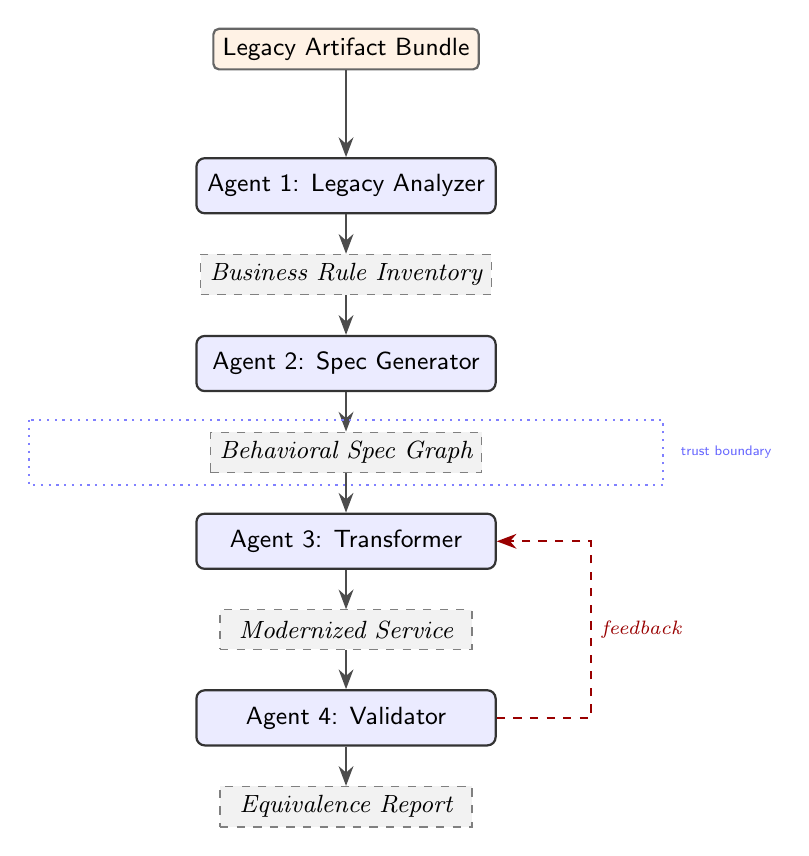
\begin{tikzpicture}[
  node distance=1.1cm and 0.5cm,
  agent/.style={rectangle, draw=black!80, fill=blue!8, thick, rounded corners=3pt,
                minimum width=3.8cm, minimum height=0.7cm, font=\small\sffamily},
  artifact/.style={rectangle, draw=black!50, fill=gray!10, dashed,
                   minimum width=3.2cm, minimum height=0.5cm, font=\small\itshape},
  input/.style={rectangle, draw=black!60, fill=orange!10, thick, rounded corners=2pt,
                minimum width=3.2cm, minimum height=0.5cm, font=\small\sffamily},
  arr/.style={-{Stealth[length=2.5mm]}, thick, black!70},
  farr/.style={-{Stealth[length=2.5mm]}, thick, red!60!black, dashed},
]
% Input
\node[input] (input) {Legacy Artifact Bundle};

% Agent 1
\node[agent, below=of input] (a1) {Agent 1: Legacy Analyzer};
\node[artifact, below=0.5cm of a1] (bri) {Business Rule Inventory};

% Agent 2
\node[agent, below=0.5cm of bri] (a2) {Agent 2: Spec Generator};
\node[artifact, below=0.5cm of a2] (bsg) {Behavioral Spec Graph};

% Agent 3
\node[agent, below=0.5cm of bsg] (a3) {Agent 3: Transformer};
\node[artifact, below=0.5cm of a3] (code) {Modernized Service};

% Agent 4
\node[agent, below=0.5cm of code] (a4) {Agent 4: Validator};
\node[artifact, below=0.5cm of a4] (report) {Equivalence Report};

% Forward arrows
\draw[arr] (input) -- (a1);
\draw[arr] (a1) -- (bri);
\draw[arr] (bri) -- (a2);
\draw[arr] (a2) -- (bsg);
\draw[arr] (bsg) -- (a3);
\draw[arr] (a3) -- (code);
\draw[arr] (code) -- (a4);
\draw[arr] (a4) -- (report);

% Feedback loop
\draw[farr] (a4.east) -- ++(1.2,0) |- node[right, pos=0.25, font=\scriptsize\itshape, text=red!60!black] {feedback} (a3.east);

% Trust boundary annotation
\draw[thick, dotted, blue!50] ([xshift=-2.3cm, yshift=0.15cm]bsg.north west) rectangle ([xshift=2.3cm, yshift=-0.15cm]bsg.south east);
\node[font=\tiny\sffamily, blue!60, anchor=west] at ([xshift=2.4cm]bsg.east) {trust boundary};

\end{tikzpicture}%
}
\caption{AgentModernize Pipeline Architecture. Solid arrows show the forward pipeline; the dashed red arrow shows the feedback loop from the Validator to the Transformer. The BSG (dotted box) acts as a trust boundary between extraction and generation.}
\label{fig:architecture}
\end{figure}

\subsection{Legacy Artifact Bundle}

The input is a \textit{Legacy Artifact Bundle} $L = \{S, C, D, N\}$: source files $S$ (COBOL, PL/SQL, shell), configuration $C$ (JCL, parameter files, schedules), database schemas $D$ (DDL, copybook layouts), and optional documentation $N$ (runbooks, requirements).

\subsection{Agent 1: Legacy Analyzer}

The Legacy Analyzer extracts explicit rules (stated in conditionals, guards, comments) and implicit rules (inferable from code patterns, default values, exception handlers, cross-module dependencies) in three sub-phases: structural parsing (entry points, PERFORM/CALL hierarchies, file I/O, external dependencies); rule extraction (conditional logic, computations, state transitions, exception patterns), with each rule annotated by description, source location, inputs/outputs, and a high/medium/low confidence score; and constraint discovery (type restrictions, ranges, referential integrity, ordering, invariants such as ``order total equals sum of line items''). \textbf{Output:} a \textit{Business Rule Inventory (BRI)} in JSON.

\subsection{Agent 2: Specification Generator}

The Specification Generator transforms the Business Rule Inventory into a \textit{Behavioral Specification Graph (BSG)}, the core intermediate representation of AgentModernize.

\textbf{Definition 1 (Behavioral Specification Graph).} A BSG is a directed graph $G = (V, E, Pre, Post, Inv)$. $V$ is a set of \textit{operation nodes}, one per discrete business operation (``validate order'', ``calculate tax''). $E \subseteq V \times V \times L$ is a set of labeled edges carrying control flow, with label set $L = \{$\texttt{sequence}, \texttt{conditional}, \texttt{parallel}, \texttt{error}, \texttt{loop}, \texttt{branch}$\}$. $Pre$/$Post: V \rightarrow \mathcal{P}$ attach pre- and postcondition predicates to each node, and $Inv$ holds global invariants. Each node is further annotated with $inputs(v)$/$outputs(v)$ (typed data fields), $rules(v)$ (BRI rule IDs), and $error\_behavior(v)$; a data dependency $u \rightarrow v$ is implicit whenever $outputs(u) \cap inputs(v) \neq \emptyset$, so control flow lives on edges and data flow on nodes.

\textbf{Edge Labels.} The six labels map to generation patterns: \texttt{sequence} to straight-line calls, \texttt{conditional} to guarded transitions (guard stored in $Pre(v)$), \texttt{parallel} to async blocks (no data dependency), \texttt{error} to exception handlers, \texttt{loop} to \texttt{while}/\texttt{for} cycles, and \texttt{branch} to \texttt{EVALUATE}/\texttt{IF-ELSE}-style multi-way selection.

\textbf{Example (S1).} One S1 node, \texttt{ValidateDisconnectOrder} (rule BR-004, \texttt{ORDER\_VALIDATION.cob:118--142}), carries preconditions \texttt{account\_status} $\in$ \{ACTIVE, SUSPENDED\} and \texttt{order\_type = DISCONNECT}, postconditions ``suspended accounts proceed for disconnect orders; non-disconnect orders rejected for suspended,'' invariant \texttt{order\_total = sum(line\_items)}, confidence \texttt{high}---an implicit rule (suspended accounts are blocked \textit{except} for disconnect orders) that a syntax translation would lose but the BSG makes explicit before generation.

\subsection{Agent 3: Modernization Transformer}

The Transformer generates a service implementation under four principles: (1) \textit{operation-to-endpoint mapping}---each BSG node becomes a function or API endpoint; (2) \textit{contract preservation}---pre/postconditions become input validation, output assertions, and error handling; (3) \textit{data-model derivation}---node I/O annotations are aggregated into typed models (Pydantic, dataclasses); (4) \textit{flow preservation}---edge labels determine the orchestration pattern. \textbf{Output:} a \textit{Modernized Service Package} (Python/FastAPI endpoints, validated data models, orchestration, error handling, and an endpoint-to-node mapping).

\subsection{Agent 4: Equivalence Validator}

The Equivalence Validator checks the modernized implementation against the behavioral contract in the BSG. It prompts the LLM with the generated code and the BSG to produce a pytest suite (at most 15 tests, named by rule ID) covering preconditions, postconditions, invariants, and boundary values, executes the suite deterministically against the generated service, and parses the results. It does not execute the legacy program: the BSG, not the legacy code, is the oracle, so a rule missed during extraction is also missed by the Validator.

\textbf{Output:} A \textit{Behavioral Equivalence Report (BER)} containing per-test PASS/FAIL status, the overall behavioral equivalence rate, the failing test output, and the business-rule IDs inferred from test names.

\textbf{Feedback Loop:} When tests fail, the pipeline re-invokes the Modernization Transformer with a patch prompt containing the current code, the failing tests, and the raw pytest output, and instructs it to change only the failing logic. The loop runs for at most three iterations. In the default configuration the final iteration is returned; a \textit{regression-aware} variant instead returns the iteration with the highest Validator-measured pass rate, using only Validator tests and never the gold-standard tests.

\subsection{Orchestration and State Management}

The four agents are orchestrated by a LangGraph directed graph. A shared state object (legacy bundle, BRI, BSG, modern code, equivalence report, iteration counter, status) accumulates artifacts across phases, giving full traceability from source to output.

%% ============================================================
\section{Evaluation Design}

\subsection{Research Questions}

We evaluate six questions: \textbf{RQ1 (Behavioral Equivalence)}---to what extent does the pipeline preserve behavioral semantics? \textbf{RQ2 (Rule Preservation)}---how effectively are individual business rules preserved end-to-end? \textbf{RQ3 (Residual Failures)}---how many gold-standard tests remain failing, as a proxy for remediation work? \textbf{RQ4 (Component Contribution)}---how much of the result is attributable to the BSG versus to feedback? \textbf{RQ5 (BSG Quality)}---how accurately does the BSG capture the gold rules? \textbf{RQ6 (Model Sensitivity)}---how does quality vary with model capability?

\subsection{Benchmark: LegacyModernize-8}
\label{sec:benchmark}

\textbf{All eight scenarios in LegacyModernize-8 are synthetic}, hand-authored to reflect realistic legacy patterns (COBOL/PL-SQL procedures with embedded business logic, multi-step workflows, and implicit rules in exception handlers and default values) rather than sampled from production codebases. Seven scenarios are drawn from telecommunications and one from banking (S8) to test generalization beyond telecom. Each scenario is a legacy artifact bundle plus a gold-standard behavioral specification curated by a domain expert (AI-assisted drafting, human-reviewed). Table~\ref{tab:benchmark} summarizes them.

\begin{table}[htbp]
\caption{LegacyModernize-8 Benchmark Scenarios. Rules column gives total (explicit/implicit) gold-standard rules; across the benchmark, 64 of 106 are explicit.}
\label{tab:benchmark}
\centering
\footnotesize
\begin{tabular}{@{}clllcc@{}}
\toprule
\textbf{ID} & \textbf{Scenario} & \textbf{Domain} & \textbf{Complexity} & \textbf{Rules (E/I)} & \textbf{Lines} \\
\midrule
S1 & Order Validation & Orders & Medium & 12 (7/5) & 346 \\
S2 & Billing Disputes & Billing & High & 12 (8/4) & 216 \\
S3 & Service Activation & Provisioning & High & 14 (8/6) & 273 \\
S4 & Circuit Inventory & Inventory & High & 13 (9/4) & 310 \\
S5 & Fault Escalation & Fault Mgmt & High & 13 (8/5) & 249 \\
S6 & Contract Renewal & Contracts & High & 12 (7/5) & 233 \\
S7 & Account Migration & Accounts & Very High & 15 (9/6) & 318 \\
S8 & Bank Transactions & Banking & Very High & 15 (8/7) & 400 \\
\bottomrule
\end{tabular}
\end{table}

Each scenario contains explicitly documented rules plus at least three implicit rules inferable only from code patterns; complexity reflects conditional branches, external dependencies, and state transitions. S1--S7 cover telecom: multi-step validation, tiered billing, capacity management, parent--child lifecycles, SLA escalation, discount stacking, and multi-phase migration with rollback. S8 is a banking transaction processor (multi-type transactions, tier limits, overdraft protection, fraud checks, dormant accounts).

\textbf{Gold-Standard Construction.} Each scenario was fixed before any pipeline run: legacy code, a rule specification, and a reference implementation for the fair-evaluation test generator. Rules were LLM-drafted (GPT-4o enumerated candidates from the source), then manually reviewed and filtered by the first author; we kept only rules a naive translation could plausibly get wrong (thresholds, exemptions, state-dependent branches, ordering, cross-field invariants, error policies), removing 4--9 candidates per scenario. Each retained rule is labeled \texttt{explicit} or \texttt{implicit}; single-annotator authorship is a threat (Section~\ref{sec:threats}).

\subsection{Metrics}

The primary metric is \textbf{Behavioral Equivalence Rate (BER)}: the fraction of gold-standard tests that pass against the generated code, $BER = |passing|/|total|$. Tests are \emph{not} derived from the BSG; they are synthesized at evaluation time by GPT-4o-mini from the gold-standard specification and each method's own code, so every method is probed through its own API surface while the same underlying rules are tested for all. Assertions execute deterministically under pytest. Because each gold rule maps to one test, the rule-level preservation score (BRPS) equals BER per scenario; we report BER only.

\subsection{Baselines}

\textbf{B1 --- Single-Prompt (SP-LLM):} one prompt containing the full legacy bundle; no intermediate representation, no verification. \textbf{B2 --- Chain-of-Thought (CoT-LLM):} one prompt with ``analyze, then design, then implement'' instructions. \textbf{B3 --- AM-NoFB:} the full pipeline with feedback disabled. \textbf{B4 --- Feedback-Only (FB-LLM):} single prompt plus the \emph{same} iterative loop as AgentModernize (3-iteration budget, patch-style repair), but no BRI/BSG---repair tests are generated from the legacy code directly. B4 isolates the specification's contribution from feedback's: the ablation missing from the earlier version of this study.

\subsection{Implementation Details}

All agents use GPT-4o-mini (OpenAI, resolving to snapshot \texttt{gpt-4o-mini-2024-07-18}) as the LLM backend. The pipeline is orchestrated using LangGraph (Python) for stateful execution. Test cases are executed using pytest. Legacy artifacts are written in COBOL/PL-SQL; modernized output targets Python (FastAPI). Temperature is set to 0.2 for extraction/specification agents and 0.0 for code generation and test generation. The feedback loop runs for a maximum of 3 iterations.

\textbf{Prompt development protocol.} All pipeline and baseline prompts were developed and tuned on S1--S7 before S8 (the banking scenario) was authored; S8 is therefore the only scenario for which prompts had not seen the domain. Gold standards were finalized before the first evaluation run and were never modified afterward. This ordering is disclosed because it means S1--S7 results carry a tuning bias (Section~\ref{sec:threats}).

\textbf{Generation draws.} Each method produces \emph{one} generated program per scenario; the three evaluation trials re-sample only the generated test suite, not the program. Consequently a BER cell is a single code-generation draw measured three ways, not an average over independent generations (Table~\ref{tab:reproducibility}). We report a second, independent regeneration in Section~\ref{sec:regeneration} and treat it as the primary result because the first pass proved unrepresentative.

\begin{table}[htbp]
\caption{Reproducibility Details}
\label{tab:reproducibility}
\centering
\footnotesize
\begin{tabular}{@{}lp{5.6cm}@{}}
\toprule
\textbf{Item} & \textbf{Details} \\
\midrule
Repository & [anonymized for double-blind review] \\
Environment & Python 3.11, LangGraph, pytest, OpenAI SDK \\
Model & GPT-4o-mini (\texttt{-2024-07-18}); temp 0.2 extract / 0.0 gen \\
Protocol & 1 code draw $\times$ 3 test-generation trials \\
Run & \texttt{run\_experiment.py}; \texttt{run\_fair\_eval\_existing.py --trials 3} \\
Output & \texttt{fair\_eval\_summary\_\{sid\}.json}, scenario folders \\
Cost & $\sim$\$5 for the reported run \\
\bottomrule
\end{tabular}
\end{table}

%% ============================================================
\section{Results}
\label{sec:fair-eval}

\subsection{RQ1: Behavioral Equivalence}

Table~\ref{tab:rq1} compares behavioral equivalence rates across all scenarios and methods.

\begin{table}[htbp]
\caption{BER (\%), independent regeneration (GPT-4o-mini). Mean of 3 test-generation trials over one code draw per cell. Largest $\sigma$: 38.5 (AM, S4); 11 of 48 cells have $\sigma>0$. Bold = best per row.}
\label{tab:rq1}
\centering
\scriptsize
\begin{tabular}{@{}ccccccc@{}}
\toprule
\textbf{Scen.} & \textbf{SP-LLM} & \textbf{CoT-LLM} & \textbf{FB-LLM} & \textbf{NoFB} & \textbf{AM} & \textbf{AM-RA} \\
\midrule
S1 & \textbf{44.4} & 0.0 & 22.2 & 0.0 & 0.0 & 0.0 \\
S2 & 0.0 & 0.0 & 0.0 & 3.0 & 3.0 & \textbf{6.1} \\
S3 & 0.0 & 0.0 & 0.0 & 0.0 & 0.0 & 0.0 \\
S4 & 0.0 & 0.0 & 0.0 & 0.0 & \textbf{22.2} & 0.0 \\
S5 & 0.0 & 0.0 & 0.0 & \textbf{8.3} & 0.0 & 0.0 \\
S6 & 0.0 & 30.0 & 36.7 & 20.0 & \textbf{56.7} & 20.0 \\
S7 & 0.0 & 0.0 & 0.0 & 0.0 & 0.0 & 0.0 \\
S8 & 33.3 & 22.2 & \textbf{40.0} & 0.0 & 0.0 & 0.0 \\
\midrule
\textbf{Avg} & 9.7 & 6.5 & \textbf{12.4} & 3.9 & 10.2 & 3.3 \\
Non-zero & 2/8 & 2/8 & 3/8 & 3/8 & 3/8 & 2/8 \\
\bottomrule
\end{tabular}
\end{table}

Two findings stand out. First, \emph{no method preserves business logic well}: every configuration averages below 13\% BER, and no method is non-zero on more than 3 of 8 scenarios. Second, the specification-guided pipeline does not dominate: the feedback-only baseline FB-LLM---same model, same iteration budget, no BSG---achieves the highest mean BER (12.4\%) and the best single result on the held-out banking scenario S8 (40.0\%). AgentModernize with feedback is close behind (10.2\%) and produces the best single-scenario result in the study (S6, 56.7\%), but S6 is also the only scenario where it clearly benefits: its three non-zero cells are S4, S6, and a 3.0\% result on S2.

\textbf{Feedback helps selectively.} Feedback raises BER on S4 (0.0\%$\rightarrow$22.2\%) and S6 (20.0\%$\rightarrow$56.7\%), both cases where the first iteration had the right endpoint structure but localized errors the Validator's tests could localize. It is neutral or mildly harmful elsewhere: S2 stays flat (3.0\%) and on S5 the 8.3\% no-feedback score is lost entirely.

\textbf{Regression-aware selection fails.} AM-RA retains the iteration with the highest \emph{Validator}-measured pass rate rather than the last iteration. On S6 this policy reverts to iteration~1 (20.0\%) and discards the 56.7\% that feedback reached: the Validator's own suite ranked the weaker program higher because its tests reward agreement with a spec-derived oracle, not with the withheld gold standard. The Validator's signal is too weak to serve as a selection criterion---an instructive negative result about using model-written tests as a proxy quality metric.

\subsection{Regeneration and Variance}
\label{sec:regeneration}

An earlier single-generation run of the identical prompts produced materially higher averages (AM 23.0\%, AM-NoFB 23.9\%, SP-LLM 12.4\%, CoT-LLM 4.5\%). The independent regeneration reported above does not reproduce them: the model is the same dated snapshot, and temperatures are 0.0 for generation, but temperature~0 does not make LLM output deterministic, and each cell contains a single generated program. We therefore treat the initial run as one draw from a wide distribution rather than a refuted figure, and report the fresh run as primary because its artifacts are preserved in the repository. Two observations reinforce this reading: S4's AM cell varies from 0.0\% to 66.7\% across test-generation trials on \emph{the same generated code} ($\sigma=38.5$), and the non-zero-scenario count (2--3 of 8 per method) is within draw-to-draw noise. Single-generation-draw BER comparisons in this domain are unreliable; adequate power requires replicated generation, which we leave to future work (Section~\ref{sec:threats}).

\subsection{RQ2: Business Rule Preservation}

Rule composition is given in Table~\ref{tab:benchmark} (64 of 106 rules explicit, 42 implicit). Because each gold-standard rule maps to exactly one generated test, every passing test in Table~\ref{tab:rq1} is a preserved rule; the explicit/implicit mix shows preservation is not confined to documented behavior---e.g., S8's passing rules under FB-LLM include the implicit dormant-account constraint. The highest single-scenario preservation is AM's 56.7\% on S6 (roughly half its tested rules, spanning explicit pricing tiers and the implicit discount-stacking rule); no other method--scenario pair preserves half of a rule set.

\subsection{RQ3: Residual Behavioral Failures}

A framework that preserves more behavior should leave fewer failures for engineers to remediate. Residual failures are the complement of Table~\ref{tab:rq1}: taking the \emph{best} method per scenario, mean BER peaks at 44.4\% (S1), 6.1\% (S2), 0\% (S3), 22.2\% (S4), 8.3\% (S5), 56.7\% (S6), 0\% (S7), and 40.0\% (S8). With suites of 10--15 generated tests per scenario (test counts vary by trial; one S5 suite contained only 2), even the best-case cell leaves roughly 43--100\% of behavioral tests failing---median best-per-scenario BER is 15.3\%, i.e., $\approx$85\% residual failure on a typical scenario. S3 and S7 fail universally under every method. All tested configurations, spec-guided or not, leave the majority of behavioral remediation to engineers on this benchmark.

\subsection{RQ4: Component Contribution}

We compare six configurations to separate the contribution of the BSG from that of the feedback loop. Table~\ref{tab:rq4} summarizes Table~\ref{tab:rq1}.

\begin{table}[htbp]
\caption{Component Comparison --- Mean BER (\%) and Coverage (Fair Evaluation)}
\label{tab:rq4}
\centering
\footnotesize
\begin{tabular}{@{}lcc@{}}
\toprule
\textbf{Configuration} & \textbf{Avg BER} & \textbf{Non-zero scenarios} \\
\midrule
FB-LLM (feedback, no BSG) & \textbf{12.4} & 3/8 \\
AM (BSG + feedback) & 10.2 & 3/8 \\
SP-LLM (single prompt) & 9.7 & 2/8 \\
CoT-LLM (single prompt, CoT) & 6.5 & 2/8 \\
AM-NoFB (BSG, no feedback) & 3.9 & 3/8 \\
AM-RA (BSG + regression-aware FB) & 3.3 & 2/8 \\
\bottomrule
\end{tabular}
\end{table}

Three findings follow:

\textbf{The BSG is not the differentiator on this benchmark.} Comparing like-for-like pairs isolates the spec's contribution under identical feedback: FB-LLM (12.4\%) exceeds AM (10.2\%), and AM-NoFB (3.9\%) is the weakest feedback-free configuration---below even single-prompt SP-LLM (9.7\%). Whatever benefit the BSG confers to generation in this run is smaller than generation-draw variance and than simply iterating with a feedback loop. We do not claim the BSG hurts; with one generation draw per cell, the 2.2-point gap between FB-LLM and AM is within noise. The supportable claim is narrower and still useful: \emph{at this scale, the BSG is not necessary for the observed BER.}

\textbf{Feedback is the largest single lever---when it works.} AM-NoFB$\rightarrow$AM lifts the mean from 3.9\% to 10.2\% (+6.3 points), entirely driven by S4 (+22.2) and S6 (+36.7). FB-LLM applies the same mechanism without a spec and scores best overall. The Validator's corrections localize and fix point errors (a wrong constant, a missing branch) but cannot repair structural failures like S3's missing orchestration.

\textbf{Iteration selection needs a better signal than self-validation.} AM-RA's regression-aware policy made things worse (3.3\%): on S6 it kept iteration~1 (20.0\%) over the 56.7\% later iteration because the Validator's own tests preferred it. Self-generated tests measure agreement with the generating model's beliefs, not with ground truth; a usable selection signal likely requires held-out or gold-adjacent tests, which introduces a careful-leakage design problem we leave to future work.

\subsection{RQ5: BSG Quality}

Table~\ref{tab:rq5} evaluates the Behavioral Specification Graph as an intermediate representation by measuring how many gold-standard business rules are captured (recall) and what fraction of extracted rules correspond to real rules (precision).

\textbf{Matching Protocol.} Each BSG node carries \texttt{business\_rule\_ids} assigned by the Specification Generator during extraction. For the run reported here we computed precision and recall \emph{automatically} by comparing that ID set against the gold-standard ID set---a fully reproducible metric. An earlier generation pass scored by manual semantic matching (same trigger, same effect, regardless of wording or ID) produced comparable figures (92.3\% recall, 90.2\% precision), so the two protocols agree within a few points.

\begin{table}[htbp]
\caption{BSG Rule Extraction Quality --- Precision and Recall (\%), automatic ID matching on the reported run}
\label{tab:rq5}
\centering
\footnotesize
\begin{tabular}{@{}cccccc@{}}
\toprule
\textbf{ID} & \textbf{Gold Rules} & \textbf{BSG Rules} & \textbf{Precision} & \textbf{Recall} & \textbf{Missed} \\
\midrule
S1 & 12 & 17 & 70.6 & \textbf{100.0} & 0 \\
S2 & 12 & 10 & \textbf{100.0} & 83.3 & 2 \\
S3 & 14 & 11 & \textbf{100.0} & 78.6 & 3 \\
S4 & 13 & 13 & \textbf{100.0} & \textbf{100.0} & 0 \\
S5 & 13 & 13 & \textbf{100.0} & \textbf{100.0} & 0 \\
S6 & 12 & 15 & 80.0 & \textbf{100.0} & 0 \\
S7 & 15 & 14 & \textbf{100.0} & 93.3 & 1 \\
S8 & 15 & 16 & 93.8 & \textbf{100.0} & 0 \\
\midrule
\textbf{Avg} & 13.3 & 13.6 & \textbf{93.0} & \textbf{94.4} & 0.8 \\
\bottomrule
\end{tabular}
\end{table}

The BSG captures 94.4\% of gold-standard rules at 93.0\% precision on the reported run, including 100\% recall on the held-out banking scenario S8: extraction quality is not restricted to the telecom domain used during development. The gap between extraction (94.4\% recall) and end-to-end BER (10.2\% for AM) is the paper's central quantitative finding: the bottleneck sits almost entirely in code generation, not in understanding what the legacy system does.

Precision losses are concentrated where the extractor writes additional plausible rules the annotator excluded (S1: 70.6\%, S6: 80.0\%); recall losses are cases of rules buried in nested conditionals (S3 misses 3 of 14). The BRI-to-BSG transfer remained lossless in this run: every rule in the inventory appears on a BSG node.

\subsection{Qualitative Analysis}

\textbf{Held-Out Scenario: S8 (Banking).} The COBOL banking transaction processor (400 lines, 15 rules, the longest scenario) is where simple methods do best: FB-LLM reaches 40.0\% BER, SP-LLM 33.3\%, and CoT-LLM 22.2\%, while all three AgentModernize variants score 0.0\%. S8's self-contained transaction types align well with single-prompt generation, and on this draw the pipeline's generated service failed every test. Notably, the same pipeline run still extracted S8's rules with 100\% recall---extraction and generation decouple entirely here. S8 was authored after the prompts were frozen and is a single scenario, so we treat it as an existence proof that BSG-free methods can win, not a domain claim.

\textbf{Feedback Loop Success (S4, S6).} The two scenarios where feedback clearly earns its cost: S6 rises from 20.0\% (no feedback) to 56.7\%---the highest single result in the study---and S4 from 0.0\% to 22.2\%. In both, iteration~1 had the correct endpoint structure but localized errors (a wrong constant, a missing branch) that the Validator's tests could pinpoint. CoT-LLM's 30.0\% on S6 suggests chain-of-thought decomposition partially captures the pricing logic without any spec artifact.

\textbf{Failure Case (S3).} All methods score 0.0\%: generated code implements the individual validation functions but never wires the dependent steps together---an orchestration gap neither feedback nor BSG decomposition addresses (S7 shows the same pattern).

\subsection{RQ6: Model Sensitivity}
\label{sec:model-comparison}

A preliminary cross-model probe (GPT-4o, a code-specialized frontier model) on an earlier generation pass suggested the pipeline's benefit shrinks or inverts with stronger models, with single-prompt generation matching or beating pipeline output. However, that probe rests on the same single-generation-draw protocol whose instability Section~\ref{sec:regeneration} documents, and we could not reproduce its mini numbers on regeneration; we therefore omit the per-scenario table rather than report figures we cannot stand behind. Model sensitivity---in particular whether a frontier model's stronger first-pass code reduces the need for either the BSG or feedback---remains an open question requiring replicated generation draws to answer properly.

\textbf{Cost note.} The reported run (8 scenarios, 6 configurations, 3 evaluation trials, 1 generation draw each) cost roughly \$5 on GPT-4o-mini.

%% ============================================================
\section{Discussion}
\label{sec:discussion}

\subsection{BSGs as a Trust Boundary}
\label{sec:bsg-trust}

The BSG was our most-debated design decision and remains the most consequential artifact the pipeline produces---though not for the reason we originally expected. It creates a trust boundary: everything upstream is extraction (noisy, confidence-scored), everything downstream is generation under contract. Without it, the pipeline is a chain of LLM calls with no checkpoint: code comes out, and there is no way to localize where behavior was lost. With it, a reviewer can inspect the specification and catch extraction errors before any code exists---and, as our results show, can also confirm that extraction was \emph{not} the failure point.

The RQ5 results support this design empirically while inverting our original claim: the BSG captures 94.4\% of gold-standard rules at 93.0\% precision, yet end-to-end BER averages 10.2\% for AM. The $\approx$84-point gap between what the spec knows and what the code does confirms that generation, not extraction, is the weak link. This is also why FB-LLM matching the pipeline is not a refutation of the BSG: FB-LLM produces only code, so when it fails there is nothing to inspect, nothing to compile, and nothing to audit. The BSG's demonstrated value in this study is diagnostic and contractual, not generative.

\subsection{When the Feedback Loop Helps}
\label{sec:feedback-decisive}

Feedback is the largest single lever in the study (+6.3 mean points from AM-NoFB to AM) but it is strictly selective: all of the gain comes from S4 (+22.2) and S6 (+36.7), where iteration~1 code had the correct endpoint structure and localized point errors the Validator's tests could pinpoint. Structural failures do not yield to patching: S3 and S7 stay at 0\% under every configuration regardless of iteration count, and S5's modest 8.3\% was lost entirely.

The AM-RA failure sharpens the lesson. Selecting iterations by Validator-measured pass rate picked a worse program on S6 because the Validator's tests share the generating model's beliefs---a model that writes a bug writes a test that blesses it. Any gating mechanism needs a signal drawn from something the generator did not produce; the withheld gold-standard suite would be ideal but cannot be used at pipeline time without leaking the evaluation into the loop. Designing a leakage-free selection oracle is concrete future work.

\subsection{Statistical Power}

With $N=8$ scenarios and \emph{one generated program per cell} we cannot make strong statistical claims, and the regeneration in Section~\ref{sec:regeneration} is the practical demonstration: method rankings shifted substantially between two identical-protocol passes. Within the reported run, $\sigma$ across the 3 test-generation trials is 0.0 for 37 of 48 cells; the largest is 38.5 (AM on S4, where the same program scored 0.0\%, 66.7\%, and 0.0\% under three independently generated suites). Two distinct variance sources must not be conflated: test-sampling noise (visible in $\sigma$) and code-generation noise (invisible in $\sigma$, only measurable across generation draws). Our reported figures bound the first; only the regeneration exercises the second. Adequately powered follow-up work needs both replicated generation and a larger benchmark.

\subsection{Comparison Scope}

We compare against LLM baselines rather than commercial modernization tools (IBM Rational, Micro Focus, TSRI; GitHub Copilot's app-modernization agents; Moderne) or agentic coding systems (SWE-Agent~\cite{yang2024sweagent}, OpenHands~\cite{wang2024openhands}). The commercial tools publish no per-rule behavioral preservation metrics, so a head-to-head is infeasible without proprietary access; SWE-Agent and OpenHands target issue resolution in existing codebases rather than legacy modernization, though such an agent could serve as a generation backend inside our Transformer.

The feedback-only baseline (FB-LLM) was the ablation missing from our earlier study, and running it changed the conclusion: it scored the highest mean BER (12.4\%). The pipeline's decomposition is therefore not validated as a BER improvement over the simplest reasonable alternative---a result we report plainly. What the pipeline uniquely provides is the artifact chain (BRI $\rightarrow$ BSG $\rightarrow$ code $\rightarrow$ equivalence report); none of the baselines produce anything inspectable between source and output.

\subsection{What This Approach Cannot Do (Yet)}

We evaluated on scenarios of 216--400 lines (Table~\ref{tab:benchmark}). Enterprise estates---thousands of programs, JCL job streams, CICS transactions, shared copybooks, DB2/IMS dependencies---are orders of magnitude larger, and nothing in this benchmark validates that scale. But scale is also where the BSG stops being optional: no prompt holds an estate, so any approach must decompose, and decomposition requires somewhere for extracted semantics to live. Our Systems Analyzer already extracts CALL/COPY dependencies and file/DB contracts per program, but a flat per-program spec cannot express \emph{cross-module} contracts (program~A CALLs program~B; both share copybook~C). Enterprise application requires hierarchical BSGs that compose module-level graphs into job-chain and system-level views, plus incremental processing---the schema supports the pieces; the composition machinery is future work, and we make no claim the current pipeline handles it.

The same reasoning motivates the longer-term direction we consider most promising: the BSG as a \emph{compilation target}. If extraction is reliable (94.4\% recall) but LLM generation is the bottleneck (10.2\% BER), the natural fix is to replace free-form generation with deterministic compilation from the spec---LLM does the fuzzy extraction it is good at, a compiler produces the code. Our preliminary compiler prototype is not yet evaluated and remains future work.

%% ============================================================
\section{Threats to Validity}
\label{sec:threats}

\textbf{Internal/external validity.} All scenarios are synthetic, single-annotator gold standards (Section~\ref{sec:benchmark}); they lack production messiness. We evaluated telecom plus one banking scenario in COBOL/PL-SQL---other domains (healthcare, government) and real codebases remain untested.

\textbf{Reliability (dominant threat).} Each method generates \emph{one} program per scenario; the 3 trials re-sample only tests, so a cell is one code draw measured three ways. The independent regeneration (Sec.~\ref{sec:regeneration}) shifted rankings materially, and AM-on-S4 varies 0--66.7\% across test samplings on identical code. Temperature~0 does not guarantee determinism. Treat all few-point differences---and even the method ordering---as provisional. Some 0\% cells reflect non-executable output rather than failed logic.

\textbf{Construct validity.} Test-based verification shows absence of divergence only for tested paths; formal verification is impractical here.

\textbf{Selection bias.} The first author designed scenarios and gold rules. Prompts were frozen before S8 was authored, making it a held-out probe against prompt--scenario co-evolution, but broader authoring bias remains; an independently authored benchmark would strengthen validity.

\textbf{Model availability and LLM-as-evaluator.} Results cover one model (GPT-4o-mini \texttt{-2024-07-18}); the unreplicated cross-model probe suggested sensitivity (Sec.~\ref{sec:model-comparison}). The same model family also generates the evaluation suites---executed deterministically by pytest, which bounds bias to coverage and assertion quality, but the gold \emph{rules} are human-reviewed while the tests that operationalize them are not.

%% ============================================================
\section{Artifact Availability}

The AgentModernize framework implementation, LegacyModernize-8 benchmark scenarios (COBOL/PL/SQL source, gold-standard business rules, and behavioral test suites), BSG schema definitions, evaluation scripts, and sample prompts are available at [anonymized for double-blind review]; a de-anonymized link will be provided in the camera-ready version.

%% ============================================================
\section{AI Use Disclosure}

AI tools (OpenAI GPT-4o) were used for grammar editing and formatting assistance during manuscript preparation. All technical content, experimental design, implementation, evaluation, and analysis were performed by the authors.

%% ============================================================
\section{Conclusion}

Legacy modernization is a behavioral preservation problem, not a syntax translation problem. AgentModernize decomposes it into extraction, specification, code generation, and validation, linked by Behavioral Specification Graphs.

Under a fair per-method protocol on GPT-4o-mini---and reporting an independent regeneration after our initial numbers failed to reproduce---no configuration preserves business logic well: all six average below 13\% BER, and the best is a feedback-only baseline without any specification (FB-LLM, 12.4\%). Feedback is the largest single lever but works only on point-error scenarios (S4, S6), and selecting iterations by the Validator's own tests made results worse. The BSG itself is not the problem: it captures 94.4\% of gold-standard rules at 93.0\% precision, including 100\% recall on the held-out banking scenario. The bottleneck sits downstream, in free-form code generation.

Two conclusions follow. First, for benchmark-scale programs, an explicit spec is not yet justified by BER---a simple feedback loop suffices. Second, and more important for practice, the BSG's value is architectural rather than generative: it is the inspectable, auditable contract that makes extraction failures diagnosable, makes validation possible without trusting the generator, and is the natural compilation target for deterministic code generation. For enterprise estates that no prompt can hold, some such intermediate representation is structurally required; whether ours is the right one at that scale is the question our hierarchical-BSG and BSG-compiler work now targets.

Future work: replicated generation draws to obtain real confidence intervals; a leakage-free iteration-selection oracle; hierarchical BSGs for cross-module contracts; evaluating the BSG-to-code compiler against free-form generation; and a study of whether domain experts trust modernized code more when they can inspect the spec.

%% ============================================================
\bibliographystyle{IEEEtran}
\begin{thebibliography}{20}

\bibitem{comella2000survey}
S.~Comella-Dorda, K.~Wallnau, R.~Seacord, and J.~Robert, ``A survey of legacy system modernization approaches,'' Software Engineering Institute, Carnegie Mellon University, Tech. Rep. CMU/SEI-2000-TN-003, 2000.

\bibitem{breivold2012systematic}
H.~P.~Breivold, I.~Crnkovic, and M.~Larsson, ``A systematic review of software architecture evolution research,'' \textit{Information and Software Technology}, vol.~54, no.~1, pp.~16--40, 2012. \texttt{doi:10.1016/j.infsof.2011.08.002}

\bibitem{kazman1998requirements}
R.~Kazman, S.~G.~Woods, and S.~J.~Carri\`{e}re, ``Requirements for integrating software architecture and reengineering models: CORUM II,'' in \textit{Proc. Working Conference on Reverse Engineering (WCRE)}, 1998. \texttt{doi:10.1109/WCRE.1998.723185}

\bibitem{rugaber2004model}
S.~Rugaber and K.~Stirewalt, ``Model-driven reverse engineering,'' \textit{IEEE Software}, vol.~21, no.~4, pp.~45--53, 2004. \texttt{doi:10.1109/MS.2004.23}

\bibitem{chen2021evaluating}
M.~Chen \textit{et al.}, ``Evaluating large language models trained on code,'' \textit{arXiv preprint arXiv:2107.03374}, 2021.

\bibitem{hou2024llm4se}
C.~Hou \textit{et al.}, ``Large language models for software engineering: A systematic literature review,'' \textit{ACM Transactions on Software Engineering and Methodology}, 2024. \texttt{doi:10.1145/3695988}

\bibitem{bruneliere2014modisco}
H.~Bruneli\`{e}re, J.~Cabot, G.~Dup\'{e}, and F.~Madiot, ``MoDisco: A model driven reverse engineering framework,'' \textit{Information and Software Technology}, vol.~56, no.~8, pp.~1012--1032, 2014. \texttt{doi:10.1016/j.infsof.2014.04.007}

\bibitem{delucia2001cobol}
A.~De~Lucia, A.~R.~Fasolino, and M.~Napoli, ``An approach for reverse engineering of COBOL-based applications,'' in \textit{Proc. European Conference on Software Maintenance and Reengineering}, 2001. \texttt{doi:10.1109/CSMR.2001.914982}

\bibitem{pan2024lost}
R.~Pan \textit{et al.}, ``Lost in translation: A study of bugs introduced by large language models while translating code,'' in \textit{Proc. IEEE/ACM International Conference on Software Engineering (ICSE)}, 2024. \texttt{doi:10.1145/3597503.3639226}

\bibitem{hong2024metagpt}
S.~Hong \textit{et al.}, ``MetaGPT: Meta programming for a multi-agent collaborative framework,'' in \textit{ICLR}, 2024.

\bibitem{qian2024chatdev}
C.~Qian \textit{et al.}, ``ChatDev: Communicative agents for software development,'' in \textit{ACL}, 2024. \texttt{doi:10.18653/v1/2024.acl-long.810}

\bibitem{huang2023agentcoder}
K.~Huang \textit{et al.}, ``AgentCoder: Multi-agent-based code generation with iterative testing and optimisation,'' \textit{arXiv preprint arXiv:2312.13010}, 2023.

\bibitem{mckeeman1998differential}
W.~McKeeman, ``Differential testing for software,'' \textit{Digital Technical Journal}, vol.~10, no.~1, pp.~100--107, 1998.

\bibitem{yang2024sweagent}
J.~Yang \textit{et al.}, ``SWE-agent: Agent-computer interfaces enable automated software engineering,'' in \textit{NeurIPS}, 2024.

\bibitem{wang2024openhands}
X.~Wang \textit{et al.}, ``OpenHands: An open platform for AI software developers as generalist agents,'' \textit{arXiv preprint arXiv:2407.16741}, 2024.

\bibitem{leavens1999jml}
G.~T.~Leavens, A.~L.~Baker, and C.~Ruby, ``JML: A notation for detailed design,'' in \textit{Behavioral Specifications of Businesses and Systems}, H.~Kilov, B.~Rumpe, and I.~Simmonds, Eds.\hskip 1em Springer, pp.~175--188, 1999. \texttt{doi:10.1007/978-1-4615-5229-1\_12}

\bibitem{meyer1992dbc}
B.~Meyer, ``Applying design by contract,'' \textit{IEEE Computer}, vol.~25, no.~10, pp.~40--51, 1992. \texttt{doi:10.1109/2.161279}

\bibitem{omg2016kdm}
Object Management Group, ``Architecture-Driven Modernization: Knowledge Discovery Meta-Model (KDM), v1.4,'' OMG Standard formal/2016-02-01, 2016. Available: \url{https://www.omg.org/spec/KDM/1.4}

\bibitem{madaan2023selfrefine}
A.~Madaan \textit{et al.}, ``Self-Refine: Iterative refinement with self-feedback,'' in \textit{Advances in Neural Information Processing Systems (NeurIPS)}, 2023.

\bibitem{shinn2023reflexion}
N.~Shinn \textit{et al.}, ``Reflexion: Language agents with verbal reinforcement learning,'' in \textit{Advances in Neural Information Processing Systems (NeurIPS)}, 2023.

\end{thebibliography}

\end{document}
